
\begin{center}
    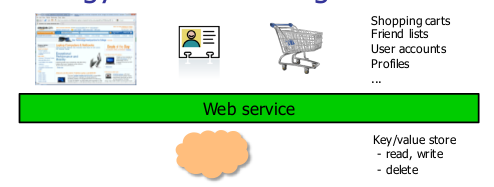
\includegraphics[width=12cm]{img/storage}
\end{center}

Many cloud services have a similar structure, 
But the actual storage service is very simple (Read/write 'blocks',
similar to a giant hard disk) and the translation done by the web service.

\paragraph{Ideal store}
\begin{itemize}
    \item Perfect durability – nothing would ever disappear in a crash
    \item 100\% availability – we could always get to the service
    \item Zero latency from anywhere on earth – no delays!
    \item Minimal bandwidth utilization – we only send across the network what we absolutely need
    \item Isolation under concurrent updates – make sure data stays consistent
\end{itemize}

BUT the “cloud” exists over a physical network (communication take time + limited bandwith)
and The “cloud” has imperfect hardware (failures)

\paragraph{Observation}
\begin{itemize}
    \item Read-­only (or read-­mostly) data is easiest to support
    \item Granularity matters: “Few large-­object” tasks generally 
        tolerate longer latencies than “many small-­object” tasks


        But it’s much more expensive to replicate or to update!

    \item[$\rightarrow$] Maybe it makes sense to develop separate solutions for large 
        read-­mostly objects vs. small read-­write objects!
        Different requirements $\rightarrow$ different technical solutions
\end{itemize}


\subsection{Key-value stores (KVS)}
The key-­value store (KVS) is a simple 
abstraction for managing persistent state where data is 
organized as (key,value) pairs with three basic operation:
\begin{enumerate}
    \item \texttt{PUT(key, value)}
    \item \texttt{value = GET(key)}
    \item \texttt{DEL(key)}
\end{enumerate}

\paragraph{Concurrency control}
Most systems use locks on individual items.



\subsubsection{Amazon dynamo}
\begin{figure}[!h]
    \centering
    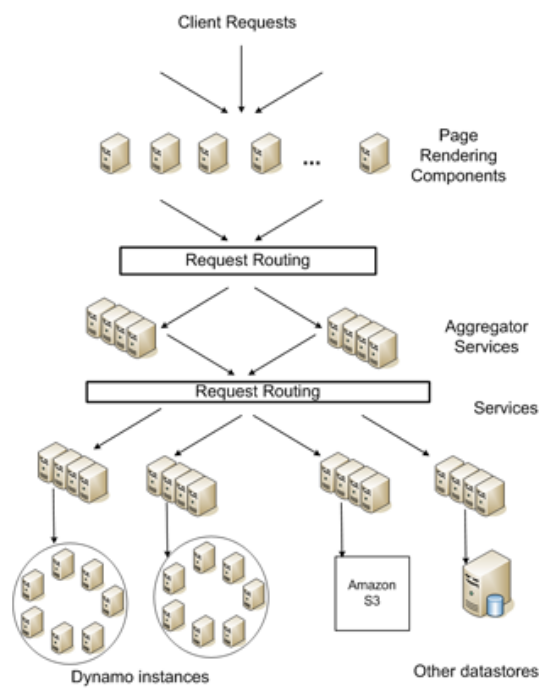
\includegraphics[width=5cm]{img/AWSplat}
    \caption{Amazon dynamo. 
        AWS is \textbf{Availability\&Partition-tolerance} and follow 
    \textbf{BASE} philosophy.}
\end{figure}

\begin{tabular}{cm{10cm}}
    Dynamo is :&
    \begin{itemize}
        \item High performance with low latency
        \item High scalable
        \item High available key storage, especially for writes
        \item Partition/fault-tolerant
        \item Eventually consistent (sacrify for high availability)
    \end{itemize}
\end{tabular}
Very low latency writes, reconciliation in reads (last write wins). Object stored are 
relatively small (typically <1MB)

\paragraph{Key Techniques}
\begin{itemize}
    \item \textbf{Consistent hashing}: dynamically partitions a set of keys
        over a set of storage nodes (hash keys and give 
        a key of m-bits). One key range per virtual node.

        \paragraph{Data partitioning and load balancing}
        A key is assigned to the closest successor node id 
        (key $k$ is assigned to the first node with $id \geq k$)
        \begin{center}
        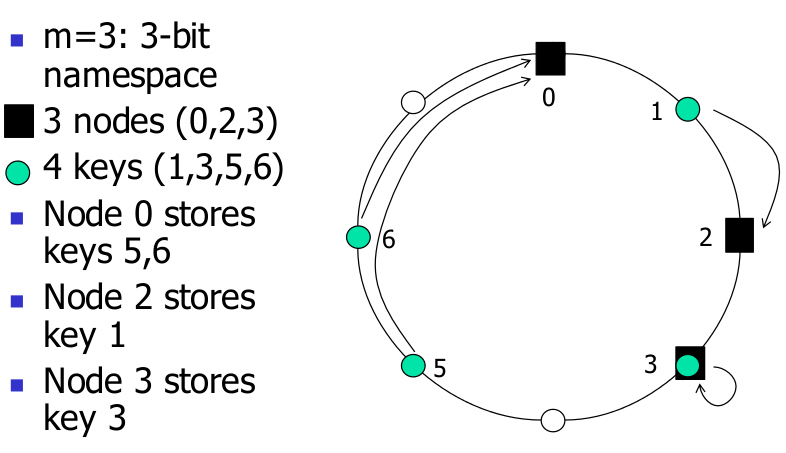
\includegraphics[width=5cm]{img/consistent}
        \end{center}

        \begin{center}
            Each node has at most $(1+\epsilon) \frac{K}{N}$ keys with $N$ nodes, $K$ keys
            and $\epsilon=O(log(N))$  To leverage heterogeneity between node ($\neq$ processing
            capabilities), Dynamo uses virtual nodes. Physical are responsible for one or more 
            virtual node depending of its capability.
            %TODO: why epsilon=0 with virtual nodes?
        \end{center}

        \paragraph{Replication}
        Replication is done on the successors node because if the node fail, it's the successor
        which will take failed node keys.

        \begin{center}
            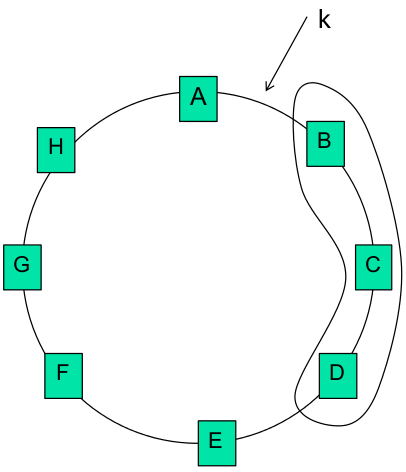
\includegraphics[width=5cm]{img/dynamoReplica}
        \end{center}

        Replication is may in asynchronous way (eventual consistency), and
        key data versioning technique is done with vector clocks.


        If the replica A in the preference list is down then
        another replica is created on a new node.
        In this case, coordinator will involve D that substitutes
        A until A comes back again. When D gets info A is
        back up it hands back the data to A


    \item \textbf{Vector clocks}: Each write to a key k is associated with a 
        vector clock VC(k) which is an array (map) of integers (one entry VC(k)[i] for each node i).

        This is use for tracking causal dependencies among different versions 
        of the same key (data)

        \begin{center}
            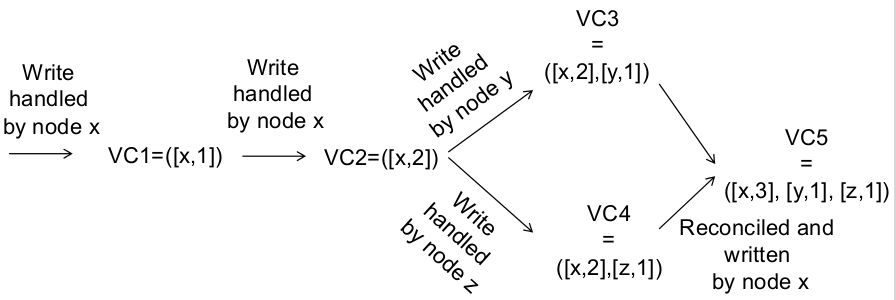
\includegraphics[width=5cm]{img/vectorClock}
        \end{center}

    \item \textbf{Sloppy quorums}: In order to enforce consistency, to response
        to a read or write operation the node must asl to a \textit{quorum}
        which is the minimum number of votes that a distributed transaction has
        to obtain.

        \begin{itemize}
            \item $R$ number of nodes that participate in a get, $W$ number
                of node that participate in a write and $R+W > N$

            \item \textbf{Put}: Generate new $VC$, write locally, send value $VC$
                to N selected nodes from preference list and wait for $W-1$

            \item \textbf{Get}: Send read to $N$ selected nodes from preference list, 
                wait for $R$, select highest versions per $VC$ and return
                all such versions. 

                Writeback merge versions.

            \item[Note]
                \begin{enumerate}
                    \item Note that each node has routing info to all other node
                        to reduce latency (but this is less scalable)
                \end{enumerate}
                To handle puts and gets, 3 differents ways:
                \begin{itemize}
				\item \textbf{Extended preference list} N nodes from preference list +
				some additional nodes (following the circle) to account for failure.
				\item \textbf{Failure-free case} Node from preference list are involved
				in get/put
				\item \textbf{Failures} First N alive nodes from extended preference list
				are involved.
			\end{itemize}
        \end{itemize}

        \textbf{Sloppy} allow availability under a much wider range of 
        partitions (failures) but sacrifice consistency. The
        N selected nodes are the first N healthy 
        nodes.

    \item \textbf{Anti-entropy protocol using hash/merkle tree}:
        Each Dynamo node keeps a Merkle tree for 
        each of its key ranges. Hash trees can be used to verify any kind of data stored.

        \begin{center}
            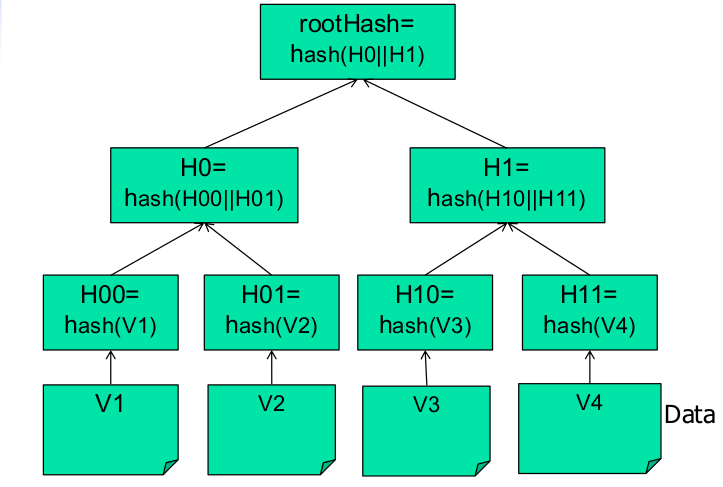
\includegraphics[width=5cm]{img/merkle}
        \end{center}

        Compares the root of the tree with replicas
        \begin{itemize}
            \item If equal, all keys in a range are equal (replicas in sync)
            \item If not equal 
                Traverse the branches of the tree to pinpoint the children that differ
                The process continues to all leaves
                Synchronize on those keys that differ
        \end{itemize}

    \item \textbf{Gossip-based group membership protocol}: 


        Membership info are also eventually 
        consistent — propagated by background 
        gossip protocol.
        \begin{itemize}
            \item Node contacts a random node every 1s
            \item 2 nodes reconcile the membership info and partitioning/placement
                metadata
        \end{itemize}


        \paragraph{Unreliable failure detection (FD)}
        Used to refresh the healthy node info in the extended 
        preference list. In the presence of steady rate of client request
        \begin{enumerate}
        	\item Node A may consider node B failed if node B
        		  does not respond to A's message
		\item Node A then uses an alternates nodes to services 
		requests that maps to B partitions
		\item A periodically checks on B
        \end{enumerate}
        If there s no client requests to drive traffic between two nodes,
        nodes are unaware whether the other has crashed or not
        \footnote{http://www.allthingsdistributed.com/2007/10/amazons\_dynamo.html}.
\end{itemize}



